% !TeX program = xelatex
\ifdefined\BookMaster\else
\documentclass[11pt,oneside]{article}
% !TeX program = xelatex
\usepackage[b5paper,left=22mm,right=22mm,top=20mm,bottom=22mm,footskip=11mm]{geometry}
\usepackage{fontspec}
\setmainfont{TeX Gyre Termes}
\setsansfont{TeX Gyre Heros}
\usepackage{amsmath,amssymb,mathtools,amsthm}
\renewcommand{\cdots}{\mathinner{\cdotp\cdotp\cdotp}}
\usepackage{graphicx,adjustbox,array,booktabs,longtable,multirow,enumitem,changepage,needspace}
\usepackage[table]{xcolor}
\usepackage{fancyhdr}
\raggedbottom
\interfootnotelinepenalty=10000
\newcommand{\BookFootnote}[2]{\begingroup\renewcommand{\thefootnote}{\fnsymbol{footnote}}\footnote[#1]{#2}\endgroup}
\newcommand{\BookFootnoteMark}[1]{\begingroup\renewcommand{\thefootnote}{\fnsymbol{footnote}}\footnotemark[#1]\endgroup}
\newcommand{\BookFootnoteText}[2]{\begingroup\renewcommand{\thefootnote}{\fnsymbol{footnote}}\footnotetext[#1]{#2}\endgroup}
\newenvironment{BookFloat}[1]{\par\addvspace{.6\baselineskip}\noindent\def\BookFloatID{#1}\begin{minipage}{\linewidth}\phantomsection\label{bookfloat:#1:start}}{\phantomsection\label{bookfloat:\BookFloatID:end}\end{minipage}\par\addvspace{.6\baselineskip}}

\usepackage[unicode,hidelinks]{hyperref}
\pagestyle{fancy}
\fancyhf{}
\newcommand{\BookFooter}{}
\fancyfoot[L]{\parbox[b]{\dimexpr\textwidth-15mm}{\footnotesize\BookFooter}}
\fancyfoot[R]{\footnotesize\thepage}
\renewcommand{\headrulewidth}{0pt}
\renewcommand{\footrulewidth}{0pt}
\setlength{\parindent}{0pt}
\setlength{\parskip}{0.2em}
\setlength{\emergencystretch}{3em}
\setlist{nosep,leftmargin=1.7em,labelsep=.65em}
\newif\ifBookNarrative
\BookNarrativetrue
\newenvironment{BookBody}{\setlength{\parindent}{0pt}}{}
\newcommand{\BookStatement}[1]{\par\addvspace{.6\baselineskip}\noindent #1\enspace\ignorespaces}
\newcommand{\BookLabel}[1]{\par\addvspace{.6\baselineskip}\needspace{3\baselineskip}\noindent\textbf{#1}\quad\ignorespaces}
\newcommand{\BookHeading}[1]{\par\addvspace{\baselineskip}\needspace{4\baselineskip}\noindent{\large\bfseries #1}\par\medskip}
\newcommand{\BookSubheading}[1]{\par\addvspace{.7\baselineskip}\needspace{3\baselineskip}\noindent{\bfseries #1}\par\smallskip}
\newcommand{\BookTextHeading}[1]{\par\addvspace{.7\baselineskip}\needspace{3\baselineskip}\noindent #1\par\smallskip}
\newcommand{\BookSectionTitle}[2]{\par\addvspace{1.2\baselineskip}\needspace{5\baselineskip}\noindent\colorbox{gray!25}{\sffamily\bfseries\small SECTION #1}\quad{\large\bfseries #2}\par\medskip}
\newcommand{\BookExerciseTitle}[1]{\par\addvspace{\baselineskip}\needspace{4\baselineskip}\noindent{\color{gray}\rule{1.5mm}{1.5mm}}\enspace{\large\bfseries Exercises #1}\par\medskip}
\newcommand{\BookBullet}[1]{\begin{list}{\textbullet}{\setlength{\leftmargin}{1.7em}\setlength{\labelwidth}{1em}\setlength{\labelsep}{.7em}\setlength{\topsep}{0pt}\setlength{\parsep}{0pt}\setlength{\itemsep}{0pt}}\item #1\end{list}}
\newcommand{\BookExercise}[2]{\begin{list}{\textbf{#1}}{\setlength{\leftmargin}{2.2em}\setlength{\labelwidth}{1.5em}\setlength{\labelsep}{.7em}\setlength{\topsep}{.15em}\setlength{\parsep}{0pt}\setlength{\itemsep}{0pt}}\item #2\end{list}}
\newcommand{\BookEnd}[1]{\unskip\nobreak\hfill\ensuremath{#1}}
\newcommand{\BookSource}[2]{\phantomsection\label{sourcepage:#1}} % Source-page anchors, retained through reflow.
\usepackage{multicol}
\usepackage{tikz}
\newcommand{\BookPartEntry}[2]{\par\noindent\makebox[17mm][l]{\bfseries Section #1}#2\par}
\newcommand{\BookPartTitle}[3]{\par\bigskip\noindent\begin{tikzpicture}\node[anchor=north west,inner sep=0pt,outer sep=0pt] (bookpart) at (0,0) {\begin{minipage}{\dimexpr\linewidth-.5pt}\hspace*{26mm}\begin{minipage}[t]{\dimexpr\linewidth-26mm}\begin{adjustbox}{max width=\linewidth}{\fontsize{20}{24}\selectfont\bfseries #2}\end{adjustbox}\par\vspace{6mm}\hrule\vspace{6mm}{\sffamily\footnotesize\setlength{\parskip}{.3em}#3}\vspace{3mm}\end{minipage}\end{minipage}};\path[shade,top color=gray!60,bottom color=white] (0,0) rectangle ([xshift=24mm]bookpart.south west);\node[anchor=north,font=\sffamily\bfseries\small] at (12mm,-2mm) {PART};\node[anchor=north,font=\sffamily\bfseries\Huge] at (12mm,-7mm) {#1};\end{tikzpicture}\par\bigskip}
\newsavebox{\BookMathBox}
\makeatletter
\newcommand{\BookInline}[1]{\leavevmode\hskip0pt\relax\begingroup\in@{\begin}{#1}\ifin@\sbox{\BookMathBox}{\(#1\)}\ifdim\wd\BookMathBox>\dimexpr\linewidth-1em\relax\resizebox{\dimexpr\linewidth-1em\relax}{!}{\usebox{\BookMathBox}}\else\(#1\)\fi\else\in@{\left}{#1}\ifin@\sbox{\BookMathBox}{\(#1\)}\ifdim\wd\BookMathBox>\dimexpr\linewidth-1em\relax\resizebox{\dimexpr\linewidth-1em\relax}{!}{\usebox{\BookMathBox}}\else\(#1\)\fi\else\(#1\)\fi\fi\endgroup\hskip0pt\relax}
\makeatother
\DeclareMathOperator{\Aut}{Aut}
\DeclareMathOperator{\End}{End}
\DeclareMathOperator{\Hom}{Hom}
\DeclareMathOperator{\GF}{GF}
\DeclareMathOperator{\irr}{irr}
\DeclareMathOperator{\lt}{lt}
\DeclareMathOperator{\lp}{lp}
\providecommand{\textcircled}[1]{\textnormal{(#1)}}

\begin{document}
\fi
\renewcommand{\BookFooter}{Section 13 Factor-Group Computations and Simple Groups}
\pdfbookmark[0]{Section 13 Factor-Group Computations and Simple Groups}{13_factor_group_computations_and_simple_groups}
\ifdefined\BookMaster\else\setcounter{page}{121}\fi
% Source PDF page 138; original printed page 121
\BookSource{138}{121}
\BookNarrativetrue

\begin{BookBody}

\BookSectionTitle{13}{Factor-Group Computations and Simple Groups}

\noindent Factor groups can be a tough topic for students to grasp. There is nothing like a bit of computation to strengthen understanding in mathematics. We start by attempting to improve our intuition concerning factor groups. Since we will be dealing with normal subgroups throughout this section, we often denote a subgroup of a group \BookInline{G} by \BookInline{N} rather than by \BookInline{H.}

Let \BookInline{N} be a normal subgroup of \BookInline{G.} In the factor group \BookInline{G/N,\allowbreak } the subgroup \BookInline{N} acts as identity element. We may regard \BookInline{N} as being\textit{ collapsed} to a single element, either to 0 in additive notation or to \BookInline{e} in multiplicative notation. This collapsing of \BookInline{N} together with the algebraic structure of \BookInline{G} require that other subsets of \BookInline{G,\allowbreak } namely, the cosets of \BookInline{N,\allowbreak } also each collapse into a single element in the factor group. A visualization of this collapsing is provided by Fig. 13.1. Recall from Theorem 12.12 that \BookInline{\gamma:G\to G/N} defined by \BookInline{\gamma (a)= } \textit{aN} for \BookInline{a\in G} is a homomorphism of \BookInline{G} onto \BookInline{G/N.} We can view the “line” \BookInline{G/N} at the bottom of Figure 13.1 as obtained by collapsing to a point each coset of \BookInline{N} in a copy of \BookInline{G.} Each point of \BookInline{G/N} thus corresponds to a whole vertical line

\begin{BookFloat}{13_factor_group_computations_and_simple_groups-p138-3}
\begin{center}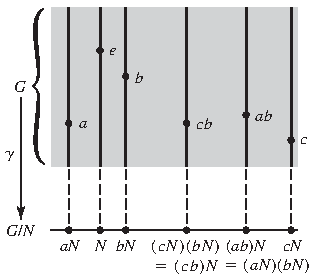
\includegraphics[width=0.429\linewidth,height=.8\textheight,keepaspectratio]{assets/p138_12.pdf}\end{center}
\begin{center}\small\textbf{13.1 Figure}\end{center}
\end{BookFloat}

\end{BookBody}

% Source PDF page 139; original printed page 122
\BookSource{139}{122}
\BookNarrativetrue

\begin{BookBody}

\noindent segment in the shaded portion, representing a coset of \BookInline{N} in \BookInline{G.} It is crucial to remember that multiplication of cosets in \BookInline{G/N} can be computed by multiplying in \BookInline{G,\allowbreak } using any representative elements of the cosets as shown in the figure.

Additively, two elements of \BookInline{G} will collapse into the same element of \BookInline{G/N} if they differ by an element of \BookInline{N.} Multiplicatively\BookInline{,\allowbreak a} and \BookInline{b} collapse together if \BookInline{ab^{- 1}} is in \BookInline{N.} The degree of collapsing can vary from nonexistent to catastrophic. We illustrate the two extreme cases by examples.

\BookLabel{13.2 Example} The trivial subgroup \BookInline{N= \{0\}} of \BookInline{\mathbb{Z}} is, of course, a normal subgroup. Compute \BookInline{\mathbb{Z}/\{0\}.}

\BookLabel{\textit{Solution}} Since \BookInline{N= \{0\}} has only one element, every coset of \BookInline{N} has only one element. That is, the cosets are of the form \BookInline{\{m\}} for \BookInline{m\in \mathbb{Z}.} There is no collapsing at all, and consequently, \BookInline{\mathbb{Z}/\{0\}\simeq \mathbb{Z}.} Each \BookInline{m\in \mathbb{Z}} is simply renamed \BookInline{\{m\}} in \BookInline{\mathbb{Z}/\{0\}.}\BookEnd{\blacktriangle}

\BookLabel{13.3 Example} Let \BookInline{n} be a positive integer. The set \BookInline{n\mathbb{R}= \{nr\mid r\in \mathbb{R}\}} is a subgroup of \BookInline{\mathbb{R}} under addition, and it is normal since \BookInline{\mathbb{R}} is abelian. Compute \BookInline{\mathbb{R}/n\mathbb{R}.}

\BookLabel{\textit{Solution}} A bit of thought shows that actually \BookInline{n\mathbb{R}= \mathbb{R},\allowbreak } because each \BookInline{x\in \mathbb{R}} is of the form \BookInline{n(x/n)} and \BookInline{x/n\in \mathbb{R}.} Thus \BookInline{\mathbb{R}/n\mathbb{R}} has only one element, the subgroup \BookInline{n\mathbb{R}.} The factor group is a trivial group consisting only of the identity element\BookInline{.}\BookEnd{\blacktriangle}

As illustrated in Examples 13.2 and 13.3 for any group \BookInline{G,\allowbreak } we have \BookInline{G/\{e\}\simeq G} and \BookInline{G/G\simeq \{e\},\allowbreak } where \BookInline{\{e\}} is the trivial group consisting only of the identity element \BookInline{e.} These two extremes of factor groups are of little importance. We would like knowledge of a factor group \BookInline{G/N} to give some information about the structure of \BookInline{G.} If \BookInline{N= \{e\},\allowbreak } the factor group has the same structure as \BookInline{G} and we might as well have tried to study \BookInline{G} directly. If \BookInline{N= G,\allowbreak } the factor group has no significant structure to supply information about \BookInline{G.} If \BookInline{G} is a finite group and \BookInline{N\neq \{e\}} is a normal subgroup of \BookInline{G,\allowbreak } then \BookInline{G/N} is a smaller group than \BookInline{G,\allowbreak } and consequently may have a more simple structure than \BookInline{G.} The multiplication of cosets in \BookInline{G/N} reflects the multiplication in \BookInline{G,\allowbreak } since products of cosets can be computed by multiplying in \BookInline{G} representative elements of the cosets.

We give two examples showing that even when \BookInline{G/N} has order 2, we may be able to deduce some useful results. If \BookInline{G} is a finite group and \BookInline{G/N} has just two elements, then we must have \BookInline{|G|= 2|N|.} Note that every subgroup \BookInline{H} containing just half the elements of a finite group \BookInline{G} must be a normal subgroup, since for each element \BookInline{a} in \BookInline{G} but not in \BookInline{H,\allowbreak } both the left coset \BookInline{aH} and the right coset \BookInline{Ha} must consist of all elements in \BookInline{G} that are not in \BookInline{H.} Thus the left and right cosets of \BookInline{H} coincide and \BookInline{H} is a normal subgroup of \BookInline{G.}

\BookLabel{13.4 Example} Because \BookInline{|S_{n}|= 2|A_{n}|,\allowbreak } we see that \BookInline{A_{n}} is a normal subgroup of \BookInline{S_{n},\allowbreak } and \BookInline{S_{n}/A_{n}} has order 2. Let \BookInline{\sigma } be an odd permutation in \BookInline{S_{n},\allowbreak } so that \BookInline{S_{n}/A_{n}= \{A_{n},\allowbreak \sigma A_{n}\}.} Renaming the element \BookInline{A_{n}} “even” and the element \BookInline{\sigma A_{n}} “odd,” the multiplication in \BookInline{S_{n}/A_{n}} shown in Table 13.5 becomes

\begin{center}\begin{adjustbox}{max width=\linewidth}\BookInline{\displaystyle \begin{aligned}(\;\text{even}\;)(\;\text{even}\;)&= \;\text{even}\;(\;\text{odd}\;)(\;\text{even}\;)= \;\text{odd}\; \\ (\;\text{even}\;)(\;\text{odd}\;)&= \;\text{odd}\;(\;\text{odd}\;)(\;\text{odd}\;)= \;\text{even}\;.\end{aligned}}\end{adjustbox}\end{center}

\begin{BookFloat}{13_factor_group_computations_and_simple_groups-p139-10}
\begin{center}\small\textbf{13.5 Table}\end{center}
\begin{center}\begin{adjustbox}{max width=\linewidth}
\renewcommand{\arraystretch}{1.2}\setlength{\tabcolsep}{5pt}
\begin{tabular}{c|c|c}
 & \BookInline{A_{n}} & \BookInline{\sigma A_{n}}\\\hline
\BookInline{A_{n}} & \BookInline{A_{n}} & \BookInline{\sigma A_{n}}\\\hline
\BookInline{\sigma A_{n}} & \BookInline{\sigma A_{n}} & \BookInline{A_{n}}\\
\end{tabular}
\end{adjustbox}\end{center}
\end{BookFloat}

\noindent Thus the factor group reflects these multiplicative properties for all the permutations in \BookInline{S_{n}.}\BookEnd{\blacktriangle}

Example 13.4 illustrates that while knowing the product of two cosets in \BookInline{G/N} does not tell us what the product of two elements of \BookInline{G} is, it may tell us that the product in \BookInline{G} of two\textit{ types} of elements is itself of a certain type.

\end{BookBody}

% Source PDF page 140; original printed page 123
\BookSource{140}{123}
\BookNarrativetrue

\begin{BookBody}

\BookLabel{13.6 Example} \textbf{(The Converse of the Theorem of Lagrange is False)} Recall that the Theorem of Lagrange states that the order of a subgroup of a finite group \BookInline{G} must divide the order of \BookInline{G.} We are now in a position to demonstrate that although the group \BookInline{A_{4}} has 12 elements and 6 divides \BookInline{12,\allowbreak A_{4}} has no subgroup of order 6.

Suppose that \BookInline{H} were a subgroup of \BookInline{A_{4}} having order 6. As observed before in Example 13.4, it would follow that \BookInline{H} would be a normal subgroup of \BookInline{A_{4}.} Then \BookInline{A_{4}/H} would have only two elements\BookInline{,\allowbreak H} and \BookInline{\sigma H} for some \BookInline{\sigma \in A_{4}} not in \BookInline{H.} Since in a group of order 2, the square of each element is the identity, we would have \BookInline{HH= H} and \BookInline{(\sigma H)(\sigma H)= H.} Now computation in a factor group can be achieved by computing with representatives in the original group. Thus, computing in \BookInline{A_{4},\allowbreak } we find that for each \BookInline{\alpha \in H} we must have \BookInline{\alpha ^{2}\in H} and for each \BookInline{\beta \in \sigma H} we must have \BookInline{\beta ^{2}\in H.} That is, the square of every element in \BookInline{A_{4}} must be in \BookInline{H.} But in \BookInline{A_{4},\allowbreak } we have

\begin{center}\begin{adjustbox}{max width=\linewidth}\BookInline{\displaystyle (1,\allowbreak 2,\allowbreak 3)= (1,\allowbreak 3,\allowbreak 2)^{2}\;\text{and}\;(1,\allowbreak 3,\allowbreak 2)= (1,\allowbreak 2,\allowbreak 3)^{2}}\end{adjustbox}\end{center}

\noindent so (1, 2, 3) and (1, 3, 2) are in \BookInline{H.} A similar computation shows that (1, 2, 4), (1, 4, 2), (1, 3, 4), (1, 4, 3), (2, 3, 4), and (2, 4, 3) are all in \BookInline{H.} This shows that there must be at least 8 elements in \BookInline{H,\allowbreak } contradicting the fact that \BookInline{H} was supposed to have order \BookInline{6.}\BookEnd{\blacktriangle}

We now turn to several examples that\textit{ compute} factor groups. If the group we start with is finitely generated and abelian, then its factor group will be also.\textit{ Computing} such a factor group means classifying it according to the fundamental theorem (Theorem 9.12 or Theorem 9.14).

\BookLabel{13.7 Example} Let us compute the factor group \BookInline{(\mathbb{Z}_{4}\times \mathbb{Z}_{6})/\langle (0,\allowbreak 1)\rangle.} Here \BookInline{\langle (0,\allowbreak 1)\rangle } is the cyclic subgroup \BookInline{H} of \BookInline{\mathbb{Z}_{4}\times \mathbb{Z}_{6}} generated by (0, 1). Thus

\begin{center}\begin{adjustbox}{max width=\linewidth}\BookInline{\displaystyle H= \{(0,\allowbreak 0),\allowbreak (0,\allowbreak 1),\allowbreak (0,\allowbreak 2),\allowbreak (0,\allowbreak 3),\allowbreak (0,\allowbreak 4),\allowbreak (0,\allowbreak 5)\}.}\end{adjustbox}\end{center}

\noindent Since \BookInline{\mathbb{Z}_{4}\times \mathbb{Z}_{6}} has 24 elements and \BookInline{H} has 6 elements, all cosets of \BookInline{H} must have 6 elements, and \BookInline{(\mathbb{Z}_{4}\times \mathbb{Z}_{6})/H} must have order 4. Since \BookInline{\mathbb{Z}_{4}\times \mathbb{Z}_{6}} is abelian, so is \BookInline{(\mathbb{Z}_{4}\times \mathbb{Z}_{6})/H(}remember, we compute in a factor group by means of representatives from the original group). In additive notation, the cosets are

\begin{center}\begin{adjustbox}{max width=\linewidth}\BookInline{\displaystyle H= (0,\allowbreak 0)+ H,\allowbreak (1,\allowbreak 0)+ H,\allowbreak (2,\allowbreak 0)+ H,\allowbreak (3,\allowbreak 0)+ H.}\end{adjustbox}\end{center}

\noindent Since we can compute by choosing the representatives (0, 0), (1, 0), (2, 0), and (3, 0), it is clear that \BookInline{(\mathbb{Z}_{4}\times \mathbb{Z}_{6})/H} is isomorphic to \BookInline{\mathbb{Z}_{4}.} Note that this is what we would expect, since in a factor group modulo \BookInline{H,\allowbreak } everything in \BookInline{H} becomes the identity element; that is, we are essentially setting everything in \BookInline{H} equal to zero. Thus the whole second factor \BookInline{\mathbb{Z}_{6}} of \BookInline{\mathbb{Z}_{4}\times \mathbb{Z}_{6}} is collapsed, leaving just the first factor \BookInline{\mathbb{Z}_{4}.}\BookEnd{\blacktriangle}

Example 13.7 is a special case of a general theorem that we now state and prove. We should acquire an intuitive feeling for this theorem in terms of\textit{ collapsing one of the} \textit{factors to the identity element}.

\BookLabel{13.8 Theorem} Let \BookInline{G= H\times K} be the direct product of groups \BookInline{H} and \BookInline{K.} Then \BookInline{H= \{(h,\allowbreak e)\mid h\in H\}} is a normal subgroup of \BookInline{G.} Also \BookInline{G/H} is isomorphic to \BookInline{K} in a natural way. Similarly, \BookInline{G/K\simeq H} in a natural way.

\BookLabel{\textit{Proof}} Consider the homomorphism \BookInline{\pi _{2}:H\times K\to K,\allowbreak } where \BookInline{\pi _{2}(h,\allowbreak k)= k.} Because Ker\BookInline{(\pi _{2})= } \BookInline{H,\allowbreak } we see that \BookInline{H} is a normal subgroup of \BookInline{H\times K.} Because \BookInline{\pi _{2}} is onto \BookInline{K,\allowbreak } Theorem 12.14 tells us that \BookInline{(H\times K)/H\simeq K.}\BookEnd{\blacklozenge}

We continue with additional computations of abelian factor groups. To illustrate how easy it is to compute in a factor group if we can compute in the whole group, we prove the following theorem.

\end{BookBody}

% Source PDF page 141; original printed page 124
\BookSource{141}{124}
\BookNarrativetrue

\begin{BookBody}

\BookLabel{13.9 Theorem} If \BookInline{G} is a cyclic group and \BookInline{N} is a subgroup of \BookInline{G,\allowbreak } then \BookInline{G/N} is cyclic.

\BookLabel{\textit{Proof}} Let \BookInline{G} be a cyclic group, so \BookInline{\langle a\rangle = G} for some \BookInline{a\in G.} Let \BookInline{N} be any subgroup of \BookInline{G.} Since \BookInline{G} is abelian\BookInline{,\allowbreak N} is a normal subgroup of \BookInline{G.} We compute the cyclic subgroup of \BookInline{G/N} generated by\textit{ aN}.

\begin{center}\begin{adjustbox}{max width=\linewidth}\BookInline{\displaystyle \langle aN\rangle = \{(aN)^{n}\mid n\in \mathbb{Z}\}= \{a^{n}N\mid n\in \mathbb{Z}\}}\end{adjustbox}\end{center}

\noindent Since \BookInline{\{a^{n}\mid n\in \mathbb{Z}\}= G,\allowbreak }

\begin{center}\begin{adjustbox}{max width=\linewidth}\BookInline{\displaystyle \{a^{n}N\mid n\in \mathbb{Z}\}= \{gN\mid g\in G\}.}\end{adjustbox}\end{center}

\noindent So \BookInline{\langle }\textit{aN}\BookInline{\rangle } contains every coset of \BookInline{G} and we see that \BookInline{G/N} is cyclic with generator \BookInline{\langle }\textit{aN}\BookInline{\rangle.} \BookEnd{\blacklozenge}

\BookLabel{13.10 Example} Let us compute the factor group \BookInline{(\mathbb{Z}_{4}\times \mathbb{Z}_{6})/\langle (0,\allowbreak 2)\rangle.} Now (0, 2) generates the subgroup

\begin{center}\begin{adjustbox}{max width=\linewidth}\BookInline{\displaystyle H= \{(0,\allowbreak 0),\allowbreak (0,\allowbreak 2),\allowbreak (0,\allowbreak 4)\}}\end{adjustbox}\end{center}

\noindent of \BookInline{\mathbb{Z}_{4}\times \mathbb{Z}_{6}} of order 3. Here the first factor \BookInline{\mathbb{Z}_{4}} of \BookInline{\mathbb{Z}_{4}\times \mathbb{Z}_{6}} is left alone. The \BookInline{\mathbb{Z}_{6}} factor, on the other hand, is essentially collapsed by a subgroup of order 3, giving a factor group in the second factor of order 2 that must be isomorphic to \BookInline{\mathbb{Z}_{2}.} Thus \BookInline{(\mathbb{Z}_{4}\times \mathbb{Z}_{6})/\langle (0,\allowbreak 2)\rangle } is isomorphic to \BookInline{\mathbb{Z}_{4}\times \mathbb{Z}_{2}.}

We can verify that \BookInline{(\mathbb{Z}_{4}\times \mathbb{Z}_{6})/\langle (0,\allowbreak 2)\rangle } is isomorphic to \BookInline{\mathbb{Z}_{4}\times \mathbb{Z}_{2}} by using Theorem 12.14. We need a homomorphism \BookInline{\phi:\mathbb{Z}_{4}\times \mathbb{Z}_{6}\to \mathbb{Z}_{4}\times \mathbb{Z}_{2}} that is onto, with kernel \BookInline{\langle (0,\allowbreak 2)\rangle.} Defining \BookInline{\phi } by \BookInline{\phi (a,\allowbreak b)= (0,\allowbreak r)} where \BookInline{r} is the remainder when \BookInline{b} is divided by 2 does the trick\BookInline{.}\BookEnd{\blacktriangle}

\BookLabel{13.11 Example} Let us compute the factor group \BookInline{(\mathbb{Z}_{4}\times \mathbb{Z}_{6})/\langle (2,\allowbreak 3)\rangle.} \textit{Be careful}! There is a great temptation to say that we are setting the 2 of \BookInline{\mathbb{Z}_{4}} and the 3 of \BookInline{\mathbb{Z}_{6}} both equal to zero, so that \BookInline{\mathbb{Z}_{4}} is collapsed to a factor group isomorphic to \BookInline{\mathbb{Z}_{2}} and \BookInline{\mathbb{Z}_{6}} to one isomorphic to \BookInline{\mathbb{Z}_{3},\allowbreak } giving a total factor group isomorphic to \BookInline{\mathbb{Z}_{2}\times \mathbb{Z}_{3}.} \textit{This is wrong}! Note that

\begin{center}\begin{adjustbox}{max width=\linewidth}\BookInline{\displaystyle H= \langle (2,\allowbreak 3)\rangle = \{(0,\allowbreak 0),\allowbreak (2,\allowbreak 3)\}}\end{adjustbox}\end{center}

\noindent is of order 2, so \BookInline{(\mathbb{Z}_{4}\times \mathbb{Z}_{6})/\langle (2,\allowbreak 3)\rangle } has order 12, not 6. Setting (2, 3) equal to zero does not make (2, 0) and (0, 3) equal to zero individually, so the factors do not collapse separately.

The possible abelian groups of order 12 are \BookInline{\mathbb{Z}_{4}\times \mathbb{Z}_{3}} and \BookInline{\mathbb{Z}_{2}\times \mathbb{Z}_{2}\times \mathbb{Z}_{3},\allowbreak } and we must decide to which one our factor group is isomorphic. These two groups are most easily distinguished in that \BookInline{\mathbb{Z}_{4}\times \mathbb{Z}_{3}} has an element of order 4, and \BookInline{\mathbb{Z}_{2}\times \mathbb{Z}_{2}\times \mathbb{Z}_{3}} does not. We claim that the coset \BookInline{(1,\allowbreak 0)+ H} is of order 4 in the factor group \BookInline{(\mathbb{Z}_{4}\times \mathbb{Z}_{6})/H.} To find the smallest power of a coset giving the identity in a factor group modulo \BookInline{H,\allowbreak } we must, by choosing representatives, find the smallest power of a representative that is in the subgroup \BookInline{H.} Now,

\begin{center}\begin{adjustbox}{max width=\linewidth}\BookInline{\displaystyle 4(1,\allowbreak 0)= (1,\allowbreak 0)+ (1,\allowbreak 0)+ (1,\allowbreak 0)+ (1,\allowbreak 0)= (0,\allowbreak 0)}\end{adjustbox}\end{center}

\noindent is the first time that (1, 0) added to itself gives an element of \BookInline{H.} Thus \BookInline{(\mathbb{Z}_{4}\times \mathbb{Z}_{6})/\langle (2,\allowbreak 3)\rangle } has an element of order 4 and is isomorphic to \BookInline{\mathbb{Z}_{4}\times \mathbb{Z}_{3}} or \BookInline{\mathbb{Z}_{12}.}

We can use Theorem 12.14 to verify that \BookInline{(\mathbb{Z}_{4}\times \mathbb{Z}_{6})/\langle (2,\allowbreak 3)\rangle } is isomorphic to \BookInline{\mathbb{Z}_{12},\allowbreak } although it is a little challenging to see what the homomorphism \BookInline{\phi:\mathbb{Z}_{4}\times \mathbb{Z}_{6}\to \mathbb{Z}_{12}} should be. We define \BookInline{\phi:\mathbb{Z}_{4}\times \mathbb{Z}_{6}\to \mathbb{Z}_{12}} by setting \BookInline{\phi (a,\allowbreak b)= 3a+ _{12}(12- 2b).} Here we interpret \BookInline{3a} and \BookInline{2b} as integer multiplication, so \BookInline{0\leq 3a<12} and \BookInline{0\leq 2b<12.} The map \BookInline{\phi } is a homomorphism, but this takes some checking, which we leave to the reader. Also, Ker\BookInline{(\phi )= \{(a,\allowbreak b)\in \mathbb{Z}_{4}\times \mathbb{Z}_{6}\mid 3a= 2b\}= \{(0,\allowbreak 0),\allowbreak (2,\allowbreak 3)\}= \langle (2,\allowbreak 3)\rangle.} We also see that \BookInline{\phi (1,\allowbreak 1)= 1,\allowbreak } which implies that \BookInline{\phi } maps onto \BookInline{\mathbb{Z}_{12}.} By the Fundamental Homomorphism Theorem\BookInline{,\allowbreak (\mathbb{Z}_{4}\times \mathbb{Z}_{6})/\langle (2,\allowbreak 3)\rangle } is isomorphic to \BookInline{\mathbb{Z}_{12}.}\BookEnd{\blacktriangle}

\end{BookBody}

% Source PDF page 142; original printed page 125
\BookSource{142}{125}
\BookNarrativetrue

\begin{BookBody}

\BookLabel{13.12 Example} Let us compute (that is, classify as in Theorem 9.12) the group \BookInline{(\mathbb{Z}\times \mathbb{Z})/\langle (1,\allowbreak 1)\rangle.} We may visualize \BookInline{\mathbb{Z}\times \mathbb{Z}} as the points in the plane with both coordinates integers, as indicated by the dots in Fig. 13.13. The subgroup \BookInline{\langle (1,\allowbreak 1)\rangle } consists of those points that lie on the \BookInline{45^{\circ }} line through the origin, indicated in the figure. The coset \BookInline{(1,\allowbreak 0)+ \langle (1,\allowbreak 1)\rangle } consists of those dots on the \BookInline{45^{\circ }} line through the point (1, 0), also shown in the figure. Continuing, we see that each coset consists of those dots lying on one of the \BookInline{45^{\circ }} lines in the figure. We may choose the representatives

\begin{center}\begin{adjustbox}{max width=\linewidth}\BookInline{\displaystyle \cdots ,\allowbreak (- 3,\allowbreak 0),\allowbreak (- 2,\allowbreak 0),\allowbreak (- 1,\allowbreak 0),\allowbreak (0,\allowbreak 0),\allowbreak (1,\allowbreak 0),\allowbreak (2,\allowbreak 0),\allowbreak (3,\allowbreak 0),\allowbreak \cdots}\end{adjustbox}\end{center}

\noindent of these cosets to compute in the factor group. Since these representatives correspond precisely to the points of \BookInline{\mathbb{Z}} on the \BookInline{x-}axis, we see that the factor group \BookInline{(\mathbb{Z}\times \mathbb{Z})/\langle (1,\allowbreak 1)\rangle } is isomorphic to \BookInline{\mathbb{Z}.}

Again, we can use the Fundamental Homomorphism Theorem as another method of computing this group. We let \BookInline{\phi:\mathbb{Z}\times \mathbb{Z}\to \mathbb{Z}} be defined by \BookInline{\phi (n,\allowbreak m)= n- m.} It is easy to verify that \BookInline{\phi } is a homomorphism\BookInline{,\allowbreak \phi } maps onto \BookInline{\mathbb{Z},\allowbreak } and Ker\BookInline{(\phi )= } \BookInline{\{(n,\allowbreak m)\in \mathbb{Z}\times \mathbb{Z}\mid n= m\}= \langle (1,\allowbreak 1)\rangle.} So by the Fundamental Homomorphism Theorem\BookInline{,\allowbreak (\mathbb{Z}\times \mathbb{Z})/\langle (1,\allowbreak 1)\rangle } is isomorphic to \BookInline{\mathbb{Z}.} Furthermore, an isomorphism is given by \BookInline{\mu ((n,\allowbreak m)+ \langle (1,\allowbreak 1)\rangle )= n- m.} This is the same isomorphism that we saw above\BookInline{.}\BookEnd{\blacktriangle}

\begin{BookFloat}{13_factor_group_computations_and_simple_groups-p142-4}
\begin{center}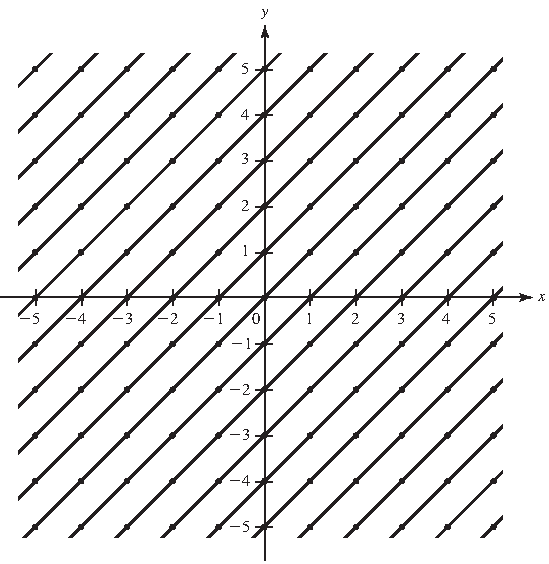
\includegraphics[width=0.752\linewidth,height=.8\textheight,keepaspectratio]{assets/p142_05.pdf}\end{center}
\begin{center}\small\textbf{13.13 Figure}\end{center}
\end{BookFloat}

\BookLabel{13.14 Example} We now compute \BookInline{(\mathbb{Z}\times \mathbb{Z})/\langle (2,\allowbreak 4)\rangle.} This is similar to Example 13.12, but there is a little twist to this one. In this example, we know that the factor group has an element with order 2, since \BookInline{(1,\allowbreak 2)\not \in \langle (2,\allowbreak 4)\rangle,\allowbreak } but \BookInline{(1,\allowbreak 2)+ (1,\allowbreak 2)\in \langle (2,\allowbreak 4)\rangle.} Furthermore\BookInline{,\allowbreak (\mathbb{Z}\times \mathbb{Z})/\langle (2,\allowbreak 4)\rangle } has an element \BookInline{(1,\allowbreak 0)+ \langle (2,\allowbreak 4)\rangle } with infinite order since \BookInline{(n,\allowbreak 0)\not \in \langle (2,\allowbreak 4)\rangle } for any \BookInline{n\in \mathbb{Z}^{+ }.} Figure 13.15 illustrates the situation. Along the line \BookInline{y= 2x} only every other lattice point is in \BookInline{\langle (2,\allowbreak 4)\rangle.} These points are filled dots in the figure. Each line with slope two contains 
% Source PDF page 143; original printed page 126
\BookSource{143}{126}
two cosets, one indicated with solid dots and one with hollow dots. Adding (1, 2) moves the solid dot cosets to the hollow dot cosets and the hollow dot cosets to the solid dot cosets while staying on the same line. Adding (0, 1) moves a coset from one line to the next. We may choose coset representatives

\end{BookBody}

\BookNarrativetrue

\begin{BookBody}

\begin{center}\begin{adjustbox}{max width=\linewidth}\BookInline{\displaystyle ...,\allowbreak (0,\allowbreak - 3),\allowbreak (0,\allowbreak - 2),\allowbreak (0,\allowbreak - 1),\allowbreak (0,\allowbreak 0),\allowbreak (0,\allowbreak 1),\allowbreak (0,\allowbreak 2),\allowbreak (0,\allowbreak 3),\allowbreak ...}\end{adjustbox}\end{center}

\noindent for the solid dot cosets and

\begin{center}\begin{adjustbox}{max width=\linewidth}\BookInline{\displaystyle ...,\allowbreak (1,\allowbreak - 3),\allowbreak (1,\allowbreak - 2),\allowbreak (1,\allowbreak - 1),\allowbreak (1,\allowbreak 0),\allowbreak (1,\allowbreak 1),\allowbreak (1,\allowbreak 2),\allowbreak (1,\allowbreak 3),\allowbreak ...}\end{adjustbox}\end{center}

\noindent for the hollow dot cosets. So it seems that we have two copies of the integers, one with a zero in the first coordinate and one with a one in the first coordinate. This leads us to guess that \BookInline{(\mathbb{Z}\times \mathbb{Z})/\langle (2,\allowbreak 4)\rangle } is isomorphic with \BookInline{\mathbb{Z}_{2}\times \mathbb{Z}.}

To verify that our guess is correct, we seek a homomorphism \BookInline{\phi:\mathbb{Z}\times \mathbb{Z}\to \mathbb{Z}_{2}\times \mathbb{Z}} that maps onto \BookInline{\mathbb{Z}_{2}\times \mathbb{Z}} and whose kernel is \BookInline{\langle (2,\allowbreak 4)\rangle.} We let \BookInline{\phi (a,\allowbreak b)= (r,\allowbreak 2a- b)} where \BookInline{r} is the remainder when \BookInline{a} is divided by 2. It is easy to check that \BookInline{\phi } is a homomorphism. Furthermore\BookInline{,\allowbreak \phi (0,\allowbreak - 1)= (0,\allowbreak 1)} and \BookInline{\phi (1,\allowbreak 2)= (1,\allowbreak 0),\allowbreak } which implies that \BookInline{\phi } maps onto \BookInline{\mathbb{Z}\times \mathbb{Z}_{2}.} It remains to compute Ker\BookInline{(\phi ).}

\begin{center}\begin{adjustbox}{max width=\linewidth}\BookInline{\displaystyle \;\text{Ker}\;(\phi )= \{(a,\allowbreak b)\mid b= 2a\;\text{and}\;a\;\text{is even}\;\}= \{(2n,\allowbreak 4n)\mid n\in \mathbb{Z}\}= \langle (2,\allowbreak 4)\rangle .}\end{adjustbox}\end{center}

\noindent Thus \BookInline{(\mathbb{Z}\times \mathbb{Z})/\langle (2,\allowbreak 4)\rangle } is isomorphic to \BookInline{\mathbb{Z}\times \mathbb{Z}_{2}} by the Fundamental Homomorphism Theorem. Furthermore, an isomorphism \BookInline{\mu:(\mathbb{Z}\times \mathbb{Z})/\langle (2,\allowbreak 4)\rangle \to \mathbb{Z}_{2}\times \mathbb{Z}} is defined by the formula \BookInline{\mu ((a,\allowbreak b)+ \langle (2,\allowbreak 4)\rangle )= (r,\allowbreak 2a- b)} where \BookInline{r} is the remainder when \BookInline{a} is divided by \BookInline{2.}\BookEnd{\blacktriangle}

\begin{BookFloat}{13_factor_group_computations_and_simple_groups-p143-8}
\begin{center}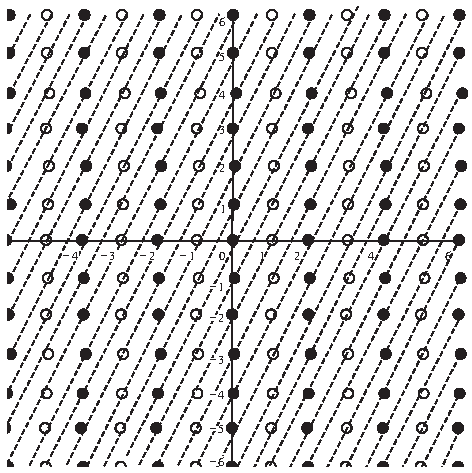
\includegraphics[width=0.647\linewidth,height=.8\textheight,keepaspectratio]{assets/p143_08.pdf}\end{center}
\begin{center}\small\textbf{13.15 Figure}\end{center}
\end{BookFloat}

\BookTextHeading{\textbf{Simple Groups}  }

\noindent As we mentioned in the preceding section, one feature of a factor group is that it gives crude information about the structure of the whole group. Of course, sometimes there may be no nontrivial proper normal subgroup. For example, Lagrange’s Theorem shows that a group of prime order can have no nontrivial proper subgroup of any sort.

\end{BookBody}

% Source PDF page 144; original printed page 127
\BookSource{144}{127}
\BookNarrativetrue

\begin{BookBody}

\BookLabel{13.16 Definition} A group is\textbf{ simple} if it is nontrivial and has no proper nontrivial normal subgroup\BookInline{.}\BookEnd{\blacksquare}

\BookLabel{13.17 Theorem} The alternating group \BookInline{A_{n}} is simple for \BookInline{n\geq 5.}

\BookLabel{\textit{Proof}} See Exercise 41. \BookEnd{\blacklozenge}

There are many simple groups other than those given above. For example\BookInline{,\allowbreak A_{5}} is of order 60 and \BookInline{A_{6}} is of order 360, and there is a simple group of nonprime order, namely 168, between these orders.

The complete determination and classification of all finite simple groups is one of the mathematical triumphs of the twentieth century. Hundreds of mathematicians worked on this task from 1950 to 1980. It can be shown that a finite group has a sort of factorization into simple groups, where the factors are unique up to order. The situation is similar to the factorization of positive integers into primes. The knowledge of all finite simple groups can be used to solve some problems of finite group theory and combinatorics.

We have seen in this text that a finite simple abelian group is isomorphic to \BookInline{\mathbb{Z}_{p}} for some prime \BookInline{p.} In 1963, Thompson and Feit [21] published their proof of a long-standing conjecture of Burnside, showing that every finite nonabelian simple group is of even order. Further great strides toward the complete classification were made by Aschbacher in the 1970s. Early in 1980, Griess announced that he had constructed a predicted “monster” simple group of order

808, 017, 424, 794, 512, 875, 886, 459, 904, 961, 710, 757, 005, 754, 368,

000, 000, 000.

\noindent Aschbacher added the final details of the classification in August 1980. The research papers contributing to the entire classification fill roughly 5000 journal pages.

We turn to the characterization of those normal subgroups \BookInline{N} of a group \BookInline{G} for which \BookInline{G/N} is a simple group. First we state an addendum to Theorem 8.5 on properties of a group homomorphism. The proof is left to Exercises 37 and 38.

\BookLabel{13.18 Theorem} Let \BookInline{\phi:G\to G^{\prime }} be a group homomorphism. If \BookInline{N} is a normal subgroup of \BookInline{G,\allowbreak } then \BookInline{\phi [N]} is a normal subgroup of \BookInline{\phi [G].} Also, if \BookInline{N^{\prime }} is a normal subgroup of \BookInline{\phi [G],\allowbreak } then \BookInline{\phi ^{- 1}[N^{\prime }]} is a normal subgroup of \BookInline{G.}\BookEnd{\blacklozenge}

Theorem 13.18 should be viewed as saying that a homomorphism \BookInline{\phi:G\to G^{\prime }} preserves normal subgroups between \BookInline{G} and \BookInline{\phi [G].} It is important to note that \BookInline{\phi [N]} may not be normal in \BookInline{G^{\prime },\allowbreak } even though \BookInline{N} is normal in \BookInline{G.} For example\BookInline{,\allowbreak \phi:\mathbb{Z}_{2}\to S_{3},\allowbreak } where \BookInline{\phi (0)= \iota } and \BookInline{\phi (1)= (1,\allowbreak 2)} is a homomorphism, and \BookInline{\mathbb{Z}_{2}} is a normal subgroup of itself, but \BookInline{\{\iota,\allowbreak (1,\allowbreak 2)\}} is not a normal subgroup of \BookInline{S_{3}.}

We can now characterize when \BookInline{G/N} is a simple group.

\BookLabel{13.19 Definition} A\textbf{ maximal normal subgroup of a group} \BookInline{G} is a normal subgroup \BookInline{M} not equal to \BookInline{G} such that there is no proper normal subgroup \BookInline{N} of \BookInline{G} properly containing \BookInline{M.}\BookEnd{\blacksquare}

\BookLabel{13.20 Theorem} \BookInline{M} is a maximal normal subgroup of \BookInline{G} if and only if \BookInline{G/M} is simple.

\BookLabel{\textit{Proof}} Let \BookInline{M} be a maximal normal subgroup of \BookInline{G.} Consider the canonical homomorphism \BookInline{\gamma:G\to G/M} given by Theorem 12.12. Now \BookInline{\gamma ^{- 1}} of any nontrivial proper normal subgroup of \BookInline{G/M} is a proper normal subgroup of \BookInline{G} properly containing \BookInline{M.} But \BookInline{M} is maximal, so this cannot happen. Thus \BookInline{G/M} is simple.

Conversely, Theorem 13.18 shows that if \BookInline{N} is a normal subgroup of \BookInline{G} properly containing \BookInline{M,\allowbreak } then \BookInline{\gamma [N]} is normal in \BookInline{G/M.} If also \BookInline{N\neq G,\allowbreak } then

\begin{center}\begin{adjustbox}{max width=\linewidth}\BookInline{\displaystyle \gamma [N]\neq  G/M\;\text{and}\;\gamma [N]\neq  \{M\}.}\end{adjustbox}\end{center}

\end{BookBody}

% Source PDF page 145; original printed page 128
\BookSource{145}{128}
\BookNarrativetrue

\begin{BookBody}

\noindent Thus, if \BookInline{G/M} is simple so that no such \BookInline{\gamma [N]} can exist, no such \BookInline{N} can exist, and \BookInline{M} is maximal\BookInline{.}\BookEnd{\blacklozenge}

\BookTextHeading{\textbf{The Center and Commutator Subgroups}  }

\noindent Every nonabelian group \BookInline{G} has two important normal subgroups, the\textit{ center} \BookInline{Z(G)} of \BookInline{G} and the\textit{ commutator subgroup} \BookInline{C} of \BookInline{G.(}The letter \BookInline{Z} comes from the German word \textit{zentrum,} meaning center.) The center \BookInline{Z(G)} is defined by

\begin{center}\begin{adjustbox}{max width=\linewidth}\BookInline{\displaystyle Z(G)= \{z\in G\mid zg= gz\;\text{for all}\;g\in G\}.}\end{adjustbox}\end{center}

\noindent Exercise 59 of Section 5 shows that \BookInline{Z(G)} is an abelian subgroup of \BookInline{G.} Since for each \BookInline{g\in } \BookInline{G} and \BookInline{z\in Z(G)} we have \BookInline{gzg^{- 1}= zgg^{- 1}= ze= z,\allowbreak } we see at once that \BookInline{Z(G)} is a normal subgroup of \BookInline{G.} If \BookInline{G} is abelian, then \BookInline{Z(G)= G;} in this case, the center is not useful.

\BookLabel{13.21 Example} The center of a group \BookInline{G} always contains the identity element \BookInline{e.} It may be that \BookInline{Z(G)= } \BookInline{\{e\},\allowbreak } in which case we say that\textbf{ the center of} \BookInline{G} \textbf{is trivial}. For example, examination of Table 4.15 for the group \BookInline{S_{3}} shows us that \BookInline{Z(S_{3})= \{\iota \},\allowbreak } so the center of \BookInline{S_{3}} is trivial. (This is a special case of Exercise 40, which shows that the center of every nonabelian group of order \BookInline{pq} for primes \BookInline{p} and \BookInline{q} is trivial.) Consequently, the center of \BookInline{S_{3}\times \mathbb{Z}_{5}} must be \BookInline{\{\iota \}\times \mathbb{Z}_{5},\allowbreak } which is isomorphic to \BookInline{\mathbb{Z}_{5}.}\BookEnd{\blacktriangle}

Turning to the commutator subgroup, recall that in forming a factor group of \BookInline{G} modulo a normal subgroup \BookInline{N,\allowbreak } we are essentially putting every element in \BookInline{G} that is in \BookInline{N} equal to \BookInline{e,\allowbreak } for \BookInline{N} forms our new identity in the factor group. This indicates another use for factor groups. Suppose, for example, that we are studying the structure of a nonabelian group \BookInline{G.} Since Theorem 9.12 gives complete information about the structure of all finitely generated abelian groups, it might be of interest to try to form an abelian group as much like \BookInline{G} as possible, an\textit{ abelianized version} of \BookInline{G,\allowbreak } by starting with \BookInline{G} and then requiring that \BookInline{ab= ba} for all \BookInline{a} and \BookInline{b} in our new group structure. To require that \BookInline{ab= ba} is to say that \BookInline{aba^{- 1}b^{- 1}= e} in our new group. An element \BookInline{aba^{- 1}b^{- 1}} in a group is a\textbf{ commutator of the group.} Thus we wish to attempt to form an abelianized version of \BookInline{G} by replacing every commutator of \BookInline{G} by \BookInline{e.} By the first observation of this paragraph, we should then attempt to form the factor group of \BookInline{G} modulo the smallest normal subgroup we can find that contains all commutators of \BookInline{G.}

\BookLabel{13.22 Theorem} Let \BookInline{G} be a group. The set of all commutators \BookInline{aba^{- 1}b^{- 1}} for \BookInline{a,\allowbreak b\in G} generates a subgroup \BookInline{C(}the\textbf{ commutator subgroup}) of \BookInline{G.} This subgroup \BookInline{C} is a normal subgroup of \BookInline{G.} Furthermore, if \BookInline{N} is a normal subgroup of \BookInline{G,\allowbreak } then \BookInline{G/N} is abelian if and only if \BookInline{C\leq N.}

\BookLabel{\textit{Proof}} The commutators certainly generate a subgroup \BookInline{C;} we must show that it is normal in \BookInline{G.} Note that the inverse \BookInline{(aba^{- 1}b^{- 1})^{- 1}} of a commutator is again a commutator, namely, \BookInline{bab^{- 1}a^{- 1}.} Also \BookInline{e= eee^{- 1}e^{- 1}} is a commutator. Theorem 7.7 then shows that \BookInline{C} consists precisely of all finite products of commutators. For \BookInline{x\in C,\allowbreak } we must show that \BookInline{g^{- 1}xg\in C} for all \BookInline{g\in G,\allowbreak } or that if \BookInline{x} is a product of commutators, so is \BookInline{g^{- 1}xg} for all \BookInline{g\in G.} By inserting \BookInline{e= gg^{- 1}} between each product of commutators occurring in \BookInline{x,\allowbreak } we see that it is sufficient to show for each commutator \BookInline{cdc^{- 1}d^{- 1}} that \BookInline{g^{- 1}(cdc^{- 1}d^{- 1})g} is in \BookInline{C.} But

\begin{center}\begin{adjustbox}{max width=\linewidth}\BookInline{\displaystyle \begin{aligned}g^{- 1}(cdc^{- 1}d^{- 1})g&= (g^{- 1}cdc^{- 1})(e)(d^{- 1}g) \\ &= (g^{- 1}cdc^{- 1})(gd^{- 1}dg^{- 1})(d^{- 1}g) \\ &= [(g^{- 1}c)d(g^{- 1}c)^{- 1}d^{- 1}][dg^{- 1}d^{- 1}g],\allowbreak \end{aligned}}\end{adjustbox}\end{center}

\noindent which is in \BookInline{C.} Thus \BookInline{C} is normal in \BookInline{G.}

\end{BookBody}

% Source PDF page 146; original printed page 129
\BookSource{146}{129}
\BookNarrativetrue

\begin{BookBody}

The rest of the theorem is obvious if we have acquired the proper feeling for factor groups. One doesn’t visualize in this way, but writing out that \BookInline{G/C} is abelian follows from

\begin{center}\begin{adjustbox}{max width=\linewidth}\BookInline{\displaystyle \begin{aligned}(aC)(bC)&= abC= ab(b^{- 1}a^{- 1}ba)C \\ &= (abb^{- 1}a^{- 1})baC= baC= (bC)(aC).\end{aligned}}\end{adjustbox}\end{center}

\noindent Furthermore, if \BookInline{N} is a normal subgroup of \BookInline{G} and \BookInline{G/N} is abelian, then \BookInline{(a^{- 1}N)(b^{- 1}N)= } \BookInline{(b^{- 1}N)(a^{- 1}N);} that is\BookInline{,\allowbreak aba^{- 1}b^{- 1}N= N,\allowbreak } so \BookInline{aba^{- 1}b^{- 1}\in N,\allowbreak } and \BookInline{C\leq N.} Finally, if \BookInline{C\leq } \BookInline{N,\allowbreak } then

\begin{center}\begin{adjustbox}{max width=\linewidth}\BookInline{\displaystyle \begin{aligned}(aN)(bN)&= abN= ab(b^{- 1}a^{- 1}ba)N \\ &= (abb^{- 1}a^{- 1})baN= baN= (bN)(aN).\end{aligned}}\end{adjustbox}\end{center} \BookEnd{\blacklozenge}

\BookLabel{13.23 Example} Using cycle notation in the symmetric group \BookInline{S_{3},\allowbreak } one commutator is

\begin{center}\begin{adjustbox}{max width=\linewidth}\BookInline{\displaystyle (1,\allowbreak 2,\allowbreak 3)(2,\allowbreak 3)(1,\allowbreak 2,\allowbreak 3)^{- 1}(2,\allowbreak 3)^{- 1}= (1,\allowbreak 2,\allowbreak 3)(2,\allowbreak 3)(1,\allowbreak 3,\allowbreak 2)(2,\allowbreak 3)= (1,\allowbreak 3,\allowbreak 2).}\end{adjustbox}\end{center}

\noindent So the commutator subgroup \BookInline{C} contains \BookInline{\langle (1,\allowbreak 3,\allowbreak 2)\rangle = A_{3},\allowbreak } the alternating group. Since \BookInline{S_{3}/A_{3}} is abelian (isomorphic with \BookInline{\mathbb{Z}_{2}),\allowbreak } Theorem 13.22 says that \BookInline{C\leq A_{3}.} Therefore\BookInline{,\allowbreak A_{3}} is the commutator subgroup\BookInline{.}\BookEnd{\blacktriangle}

\end{BookBody}

\BookNarrativefalse

\begin{BookBody}

\BookExerciseTitle{13} \BookEnd{\blacksquare}

\BookTextHeading{\textbf{Computations}}

\noindent In Exercises 1 through 14, classify the given group according to the fundamental theorem of finitely generated abelian groups.

\BookExercise{1.}{\BookInline{(\mathbb{Z}_{2}\times \mathbb{Z}_{4})/\langle (0,\allowbreak 1)\rangle }}

\BookExercise{2.}{\BookInline{(\mathbb{Z}_{2}\times \mathbb{Z}_{4})/\langle (0,\allowbreak 2)\rangle }}

\BookExercise{3.}{\BookInline{(\mathbb{Z}_{2}\times \mathbb{Z}_{4})/\langle (1,\allowbreak 2)\rangle }}

\BookExercise{4.}{\BookInline{(\mathbb{Z}_{4}\times \mathbb{Z}_{8})/\langle (1,\allowbreak 2)\rangle }}

\BookExercise{5.}{\BookInline{(\mathbb{Z}_{4}\times \mathbb{Z}_{4}\times \mathbb{Z}_{8})/\langle (1,\allowbreak 2,\allowbreak 4)\rangle }}

\BookExercise{6.}{\BookInline{(\mathbb{Z}\times \mathbb{Z})/\langle (0,\allowbreak 1)\rangle }}

\BookExercise{7.}{\BookInline{(\mathbb{Z}\times \mathbb{Z})/\langle (0,\allowbreak 2)\rangle }}

\BookExercise{8.}{\BookInline{(\mathbb{Z}\times \mathbb{Z}\times \mathbb{Z})/\langle (1,\allowbreak 1,\allowbreak 1)\rangle }}

\BookExercise{9.}{\BookInline{(\mathbb{Z}\times \mathbb{Z}\times \mathbb{Z}_{4})/\langle (3,\allowbreak 0,\allowbreak 0)\rangle }}

\BookExercise{10.}{\BookInline{(\mathbb{Z}\times \mathbb{Z}\times \mathbb{Z}_{8})/\langle (0,\allowbreak 4,\allowbreak 0)\rangle }}

\BookExercise{11.}{\BookInline{(\mathbb{Z}\times \mathbb{Z})/\langle (2,\allowbreak 2)\rangle }}

\BookExercise{12.}{\BookInline{(\mathbb{Z}\times \mathbb{Z}\times \mathbb{Z})/\langle (3,\allowbreak 3,\allowbreak 3)\rangle }}

\BookExercise{13.}{\BookInline{(\mathbb{Z}\times \mathbb{Z})/\langle (2,\allowbreak 6)\rangle }}

\BookExercise{14.}{\BookInline{(\mathbb{Z}\times \mathbb{Z}\times \mathbb{Z}_{2})/\langle (1,\allowbreak 1,\allowbreak 1)\rangle }}

\BookExercise{15.}{Find both the center and the commutator subgroup of \BookInline{D_{4}.}}

\BookExercise{16.}{Find both the center and the commutator subgroup of \BookInline{\mathbb{Z}_{3}\times S_{3}.}}

\BookExercise{17.}{Find both the center and the commutator subgroup of \BookInline{S_{3}\times D_{4}.}}

\BookExercise{18.}{Describe all subgroups of order \BookInline{\leq 4} of \BookInline{\mathbb{Z}_{4}\times \mathbb{Z}_{4},\allowbreak } and in each case classify the factor group of \BookInline{\mathbb{Z}_{4}\times \mathbb{Z}_{4}} modulo the subgroup by Theorem 9.12. That is, describe the subgroup and say that the factor group of \BookInline{\mathbb{Z}_{4}\times \mathbb{Z}_{4}} modulo the subgroup is isomorphic to \BookInline{\mathbb{Z}_{2}\times \mathbb{Z}_{4},\allowbreak } or whatever the case may be. [\textit{Hint}\BookInline{:\mathbb{Z}_{4}\times \mathbb{Z}_{4}} has six different cyclic subgroups of order 4. Describe them by giving a generator, such as the subgroup \BookInline{\langle (1,\allowbreak 0)\rangle.} There is one subgroup of order 4 that is isomorphic to the Klein 4-group. There are three subgroups of order 2.]}

\BookTextHeading{\textbf{Concepts}}

\noindent In Exercises 19 and 20, correct the definition of the italicized term without reference to the text, if correction is needed, so that it is in a form acceptable for publication.

\BookExercise{19.}{The\textit{ center} of a group \BookInline{G} contains all elements of \BookInline{G} that commute with every element of \BookInline{G.}}

\BookExercise{20.}{The\textit{ commutator subgroup} of a group \BookInline{G} is \BookInline{\{a^{- 1}b^{- 1}ab\mid a,\allowbreak b\in G\}.}}

\end{BookBody}

% Source PDF page 147; original printed page 130
\BookSource{147}{130}
\BookNarrativefalse

\begin{BookBody}

\BookExercise{21.}{Determine whether each of following is true or false.}

\BookExercise{a.}{Every factor group of a cyclic group is cyclic.}

\BookExercise{b.}{A factor group of a noncyclic group is again noncyclic.}

\BookExercise{c.}{\textbf{c}\BookInline{.\mathbb{R}/\mathbb{Z}} under addition has no element of order 3.}

\BookExercise{d.}{\textbf{d}\BookInline{.\mathbb{R}/\mathbb{Q}} under addition has no element of order 2.}

\BookExercise{e.}{\textbf{e}\BookInline{.\mathbb{R}/\mathbb{Z}} under addition has an infinite number of elements of order 4.}

\BookExercise{f.}{If the commutator subgroup \BookInline{C} of a group \BookInline{G} is \BookInline{\{e\},\allowbreak } then \BookInline{G} is abelian.}

\BookExercise{g.}{If \BookInline{G/H} is abelian, then the commutator subgroup \BookInline{C} of \BookInline{G} contains \BookInline{H.}}

\BookExercise{h.}{The commutator subgroup of a simple group \BookInline{G} must be \BookInline{G} itself.}

\BookExercise{i.}{The commutator subgroup of a nonabelian simple group \BookInline{G} must be \BookInline{G} itself.}

\BookExercise{j.}{All nontrivial finite simple groups have prime order.}

\noindent In Exercises 22 through 25, let \BookInline{F} be the additive group of all functions mapping \BookInline{\mathbb{R}} into \BookInline{\mathbb{R},\allowbreak } and let \BookInline{F^{\ast }} be the multiplicative group of all elements of \BookInline{F} that do not assume the value 0 at any point of \BookInline{\mathbb{R}.}

\BookExercise{22.}{Let \BookInline{K} be the subgroup of \BookInline{F} consisting of the constant functions. Find a subgroup of \BookInline{F} to which \BookInline{F/K} is isomorphic.}

\BookExercise{23.}{Let \BookInline{K^{\ast }} be the subgroup of \BookInline{F^{\ast }} consisting of the nonzero constant functions. Find a subgroup of \BookInline{F^{\ast }} to which \BookInline{F^{\ast }/K^{\ast }} is isomorphic.}

\BookExercise{24.}{Let \BookInline{K} be the subgroup of continuous functions in \BookInline{F.} Can you find an element of \BookInline{F/K} having order 2? Why or why not?}

\BookExercise{25.}{Let \BookInline{K^{\ast }} be the subgroup of \BookInline{F^{\ast }} consisting of the continuous functions in \BookInline{F^{\ast }.} Can you find an element of \BookInline{F^{\ast }/K^{\ast }} having order 2? Why or why not?}

\noindent In Exercises 26 through 28, let \BookInline{U} be the multiplicative group \BookInline{\{ z \in \mathbb { C } \big | | z | = 1 \}}.

\BookExercise{26.}{Let \BookInline{z_{0}\in U.} Show that \BookInline{z_{0}U= \{z_{0}z\mid z\in U\}} is a subgroup of \BookInline{U,\allowbreak } and compute \BookInline{U/z_{0}U.}}

\BookExercise{27.}{To what group we have mentioned in the text is \BookInline{U/\langle - 1\rangle } isomorphic?}

\BookExercise{28.}{Let \BookInline{\zeta _{n}= } cos\BookInline{(2\pi /n)+ i} sin\BookInline{(2\pi /n)} where \BookInline{n\in \mathbb{Z}^{+ }.} To what group we have mentioned is \BookInline{U/\langle \zeta _{n}\rangle } isomorphic?}

\BookExercise{29.}{To what group mentioned in the text is the additive group \BookInline{\mathbb{R}/\mathbb{Z}} isomorphic?}

\BookExercise{30.}{Give an example of a group \BookInline{G} having no elements of finite order greater than 1 and a normal subgroup \BookInline{H\unlhd G,\allowbreak } \BookInline{H\neq G,\allowbreak } so that in \BookInline{G/H} every element has finite order.}

\BookExercise{31.}{Let \BookInline{H} and \BookInline{K} be normal subgroups of a group \BookInline{G.} Give an example showing that we may have \BookInline{H\simeq K} while \BookInline{G/H} is not isomorphic to \BookInline{G/K.}}

\BookExercise{32.}{Describe the center of every simple}

\BookExercise{a.}{abelian group}

\BookExercise{b.}{nonabelian group.}

\BookExercise{33.}{Describe the commutator subgroup of every simple}

\BookExercise{a.}{abelian group}

\BookExercise{b.}{nonabelian group.}

\BookLabel{\textit{Proof}} \textbf{ Synopsis}

\BookExercise{34.}{Give a one-sentence synopsis of the proof of Theorem 13.9.}

\BookExercise{35.}{Give at most a two-sentence synopsis of the proof of Theorem 13.20.}

\BookTextHeading{\textbf{Theory}}

\BookExercise{36.}{Show that if a finite group \BookInline{G} contains a nontrivial subgroup of index 2 in \BookInline{G,\allowbreak } then \BookInline{G} is not simple.}

\BookExercise{37.}{Let \BookInline{\phi:G\to G^{\prime }} be a group homomorphism, and let \BookInline{N} be a normal subgroup of \BookInline{G.} Show that \BookInline{\phi [N]} is a normal subgroup of \BookInline{\phi [G].}}

\end{BookBody}

% Source PDF page 148; original printed page 131
\BookSource{148}{131}
\BookNarrativefalse

\begin{BookBody}

\BookExercise{38.}{Let \BookInline{\phi:G\to G^{\prime }} be a group homomorphism, and let \BookInline{N^{\prime }} be a normal subgroup of \BookInline{G^{\prime }.} Show that \BookInline{\phi ^{- 1}[N^{\prime }]} is a normal subgroup of \BookInline{G.}}

\BookExercise{39.}{Show that if \BookInline{G} is nonabelian, then the factor group \BookInline{G/Z(G)} is not cyclic. [\textit{Hint:} Show the equivalent contrapositive, namely, that if \BookInline{G/Z(G)} is cyclic then \BookInline{G} is abelian (and hence \BookInline{Z(G)= G).]}}

\BookExercise{40.}{Using Exercise 39, show that a nonabelian group \BookInline{G} of order \BookInline{pq} where \BookInline{p} and \BookInline{q} are primes has a trivial center.}

\BookExercise{41.}{Prove that \BookInline{A_{n}} is simple for \BookInline{n\geq 5,\allowbreak } following the steps and hints given.}

\BookExercise{a.}{Show \BookInline{A_{n}} contains every 3-cycle if \BookInline{n\geq 3.}}

\BookExercise{b.}{Show \BookInline{A_{n}} is generated by the 3-cycles for \BookInline{n\geq 3.[}\textit{Hint:} Note that \BookInline{(a,\allowbreak b)(c,\allowbreak d)= (a,\allowbreak c,\allowbreak b)(a,\allowbreak c,\allowbreak d)} and \BookInline{(a,\allowbreak c)(a,\allowbreak b)= (a,\allowbreak b,\allowbreak c).]}}

\BookExercise{c.}{Let \BookInline{r} and \BookInline{s} be fixed elements of \BookInline{\{1,\allowbreak 2,\allowbreak \cdots,\allowbreak n\}} for \BookInline{n\geq 3.} Show that \BookInline{A_{n}} is generated by the \BookInline{n} “special” 3cycles of the form \BookInline{(r,\allowbreak s,\allowbreak i)} for \BookInline{1\leq i\leq n[}\textit{Hint:} Show every 3-cycle is the product of “special” 3-cycles by computing}

\begin{center}\begin{adjustbox}{max width=\linewidth}\BookInline{\displaystyle (r,\allowbreak s,\allowbreak i)^{2},\allowbreak (r,\allowbreak s,\allowbreak j)(r,\allowbreak s,\allowbreak i)^{2},\allowbreak (r,\allowbreak s,\allowbreak j)^{2}(r,\allowbreak s,\allowbreak i),\allowbreak }\end{adjustbox}\end{center}

and

\begin{center}\begin{adjustbox}{max width=\linewidth}\BookInline{\displaystyle (r,\allowbreak s,\allowbreak i)^{2}(r,\allowbreak s,\allowbreak k)(r,\allowbreak s,\allowbreak j)^{2}(r,\allowbreak s,\allowbreak i).}\end{adjustbox}\end{center}

Observe that these products give all possible types of 3-cycles.]

\BookExercise{d.}{Let \BookInline{N} be a normal subgroup of \BookInline{A_{n}} for \BookInline{n\geq 3.} Show that if \BookInline{N} contains a 3-cycle, then \BookInline{N= A_{n}.[}\textit{Hint:} Show that \BookInline{(r,\allowbreak s,\allowbreak i)\in N} implies that \BookInline{(r,\allowbreak s,\allowbreak j)\in N} for \BookInline{j= 1,\allowbreak 2,\allowbreak \cdots,\allowbreak n} by computing}

\begin{center}\begin{adjustbox}{max width=\linewidth}\BookInline{\displaystyle ((r,\allowbreak s)(i,\allowbreak j))(r,\allowbreak s,\allowbreak i)^{2}((r,\allowbreak s)(i,\allowbreak j))^{- 1}.]}\end{adjustbox}\end{center}

\BookExercise{e.}{Let \BookInline{N} be a nontrivial normal subgroup of \BookInline{A_{n}} for \BookInline{n\geq 5.} Show that one of the following cases must hold, and conclude in each case that \BookInline{N= A_{n}.}}

\textbf{Case I} \BookInline{N} contains a 3-cycle.

\textbf{Case II} \BookInline{N} contains a product of disjoint cycles, at least one of which has length greater than 3. [\textit{Hint:} Suppose \BookInline{N} contains the disjoint product \BookInline{\sigma = \mu (a_{1},\allowbreak a_{2},\allowbreak \cdots,\allowbreak a_{r}).} Show \BookInline{\sigma ^{- 1}(a_{1},\allowbreak a_{2},\allowbreak a_{3})\sigma (a_{1},\allowbreak a_{2},\allowbreak a_{3})^{- 1}} is in \BookInline{N,\allowbreak } and compute it.]

\textbf{Case III} \BookInline{N} contains a disjoint product of the form \BookInline{\sigma = \mu (a_{4},\allowbreak a_{5},\allowbreak a_{6})(a_{1},\allowbreak a_{2},\allowbreak a_{3}).[}\textit{Hint:} Show \BookInline{\sigma ^{- 1}(a_{1},\allowbreak a_{2},\allowbreak a_{4})} \BookInline{\sigma (a_{1},\allowbreak a_{2},\allowbreak a_{4})^{- 1}} is in \BookInline{N,\allowbreak } and compute it.]

\textbf{Case IV} \BookInline{N} contains a disjoint product of the form \BookInline{\sigma = \mu (a_{1},\allowbreak a_{2},\allowbreak a_{3})} where \BookInline{\mu } is a product of disjoint 2cycles. [\textit{Hint:} Show \BookInline{\sigma ^{2}\in N} and compute it.]

\textbf{Case V} \BookInline{N} contains a disjoint product \BookInline{\sigma } of the form \BookInline{\sigma = \mu (a_{3},\allowbreak a_{4})(a_{1},\allowbreak a_{2}),\allowbreak } where \BookInline{\mu } is a product of an even number of disjoint 2-cycles. [\textit{Hint:} Show that \BookInline{\sigma ^{- 1}(a_{1},\allowbreak a_{2},\allowbreak a_{3})\sigma (a_{1},\allowbreak a_{2},\allowbreak a_{3})^{- 1}} is in \BookInline{N,\allowbreak } and compute it to deduce that \BookInline{\alpha = (a_{2},\allowbreak a_{4})(a_{1},\allowbreak a_{3})} is in \BookInline{N.} Using \BookInline{n\geq 5} for the first time, find \BookInline{i\neq a_{1},\allowbreak a_{2},\allowbreak a_{3},\allowbreak a_{4}} in \BookInline{\{1,\allowbreak 2,\allowbreak \cdots,\allowbreak n\}.} Let \BookInline{\beta = (a_{1},\allowbreak a_{3},\allowbreak i).} Show that \BookInline{\beta ^{- 1}\alpha \beta \alpha \in N,\allowbreak } and compute it.]

\BookExercise{42.}{Let \BookInline{N} be a normal subgroup of \BookInline{G} and let \BookInline{H} be any subgroup of \BookInline{G.} Let \BookInline{HN= \{hn\mid h\in H,\allowbreak n\in N\}.} Show that \BookInline{HN} is a subgroup of \BookInline{G,\allowbreak } and is the smallest subgroup containing both \BookInline{N} and \BookInline{H.}}

\BookExercise{43.}{With reference to the preceding exercise, let \BookInline{M} also be a normal subgroup of \BookInline{G.} Show that \BookInline{NM} is again a normal subgroup of \BookInline{G.}}

\BookExercise{44.}{Show that if \BookInline{H} and \BookInline{K} are normal subgroups of a group \BookInline{G} such that \BookInline{H\cap K= \{e\},\allowbreak } then \BookInline{hk= kh} for all \BookInline{h\in H} and \BookInline{k\in K.[}\textit{Hint:} Consider the commutator \BookInline{hkh^{- 1}k^{- 1}= (hkh^{- 1})k^{- 1}= h(kh^{- 1}k^{- 1}).]}}

\BookExercise{45.}{With reference to the three preceding exercises, let \BookInline{H} and \BookInline{K} be normal subgroups of a group \BookInline{G} such that \BookInline{HK= G} and \BookInline{H\cap K= \{e\}.} Prove that \BookInline{G} is isomorphic with \BookInline{H\times G.}}

\end{BookBody}
\ifdefined\BookMaster\let\BookFinish\relax\else\def\BookFinish{\end{document}}\fi\BookFinish
